\usetikzlibrary{arrows, shapes.geometric}

\tikzstyle{startstop} = [rectangle, rounded corners, minimum width=3cm, minimum height=1cm,text centered, draw=black, fill=red!30]
\tikzstyle{io} = [trapezium, trapezium left angle=70, trapezium right angle=110, minimum width=3cm, minimum height=1cm, text centered, draw=black, fill=blue!30]
\tikzstyle{process} = [rectangle, minimum width=3cm, minimum height=1cm, text centered, text width=3cm, draw=black, fill=orange!30]
\tikzstyle{decision} = [diamond, minimum width=3cm, minimum height=1cm, text centered, draw=black, fill=green!30]
\tikzstyle{arrow} = [thick,->,>=stealth]

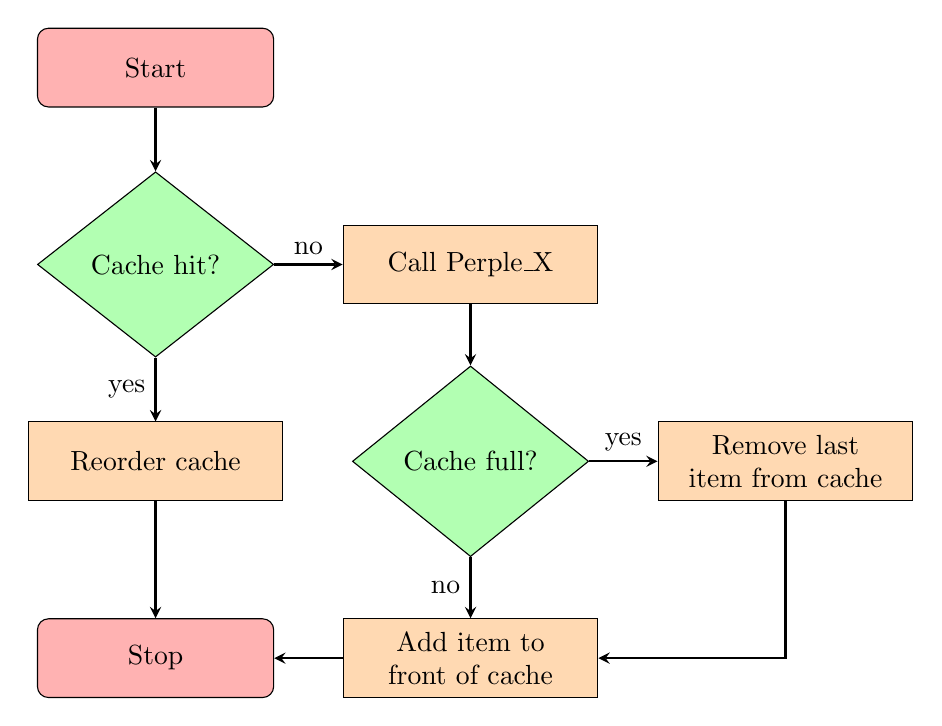
\begin{tikzpicture}[node distance=2cm]
    \node (start) [startstop] {Start};
    \node (dec1) [decision, below of=start, yshift=-0.5cm] {Cache hit?};
    \node (pro1a) [process, right of=dec1, xshift=2cm] {Call Perple\_X};
    \node (pro1b) [process, below of=dec1, yshift=-0.5cm] {Reorder cache};
    \node (dec2) [decision, below of=pro1a, yshift=-0.5cm] {Cache full?};
    \node (pro2a) [process, right of=dec2, xshift=2cm] {Remove last item from cache};
    \node (pro2b) [process, below of=dec2, yshift=-0.5cm] {Add item to front of cache};
    \node (stop) [startstop, below of=pro1b, yshift=-0.5cm] {Stop};
    
    \draw [arrow] (start) -- (dec1);
    \draw [arrow] (dec1) -- node[anchor=south] {no} (pro1a);
    \draw [arrow] (dec1) -- node[anchor=east] {yes} (pro1b);
    \draw [arrow] (pro1a) -- (dec2);
    \draw [arrow] (dec2) -- node[anchor=south] {yes} (pro2a);
    \draw [arrow] (dec2) -- node[anchor=east] {no} (pro2b);
    \draw [arrow] (pro2a) |- (pro2b);
    \draw [arrow] (pro1b) -- (stop);
    \draw [arrow] (pro2b) -- (stop);
\end{tikzpicture}